\documentclass[a4paper]{article}

\usepackage[english]{babel}
\usepackage[utf8]{inputenc}
\usepackage{amsmath}
\usepackage{amsfonts}
\usepackage{graphicx}
\usepackage{hyperref}
\usepackage[colorinlistoftodos]{todonotes}

\title{Fisher Linear Discriminant Analysis}

\author{Cheng Li, Bingyu Wang}

\date{\today}

\begin{document}
\maketitle
\section{What's LDA}


Fisher Linear Discriminant Analysis (also called Linear Discriminant Analysis(LDA)) are methods used in statistics, pattern recognition and machine learning to find a linear combination of features which characterizes or separates two or more classes of objects or events. The resulting combination may be used as a linear classifier, or, more commonly, for dimensionality reduction before later classification.

LDA is closely related to PCA, for both of them are based on linear, i.e. matrix multiplication, transformations. For the case of PCA, the transformation is baed on minimizing mean square error between original data vectors and data vectors that can be estimated fro the reduced dimensionality data vectors. And the PCA does not take into account any difference in class. But for the case of LDA, the transformation is based on maximizing a ratio of ``between-class variance" to ``within-class variance" with the goal of reducing data variation in the same class and increasing the separation between classes. Let's see an example of LDA as below(Figure\ref{fig:example}): 

\begin {figure}[h]
\centering
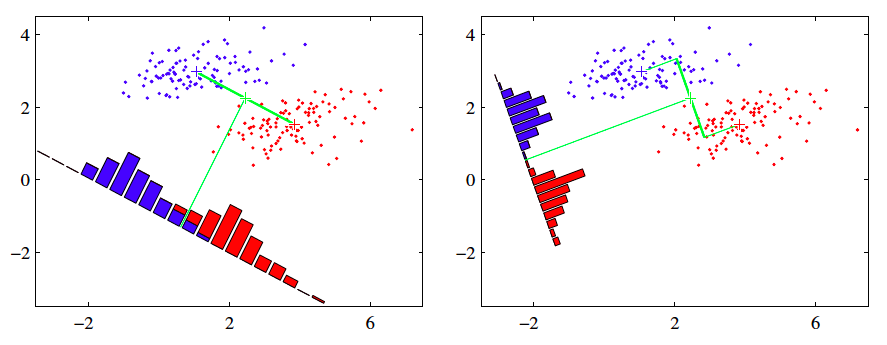
\includegraphics[width=0.7\textwidth]{./images/example.png}
\caption{\label{fig:example} LDA examples}
\medskip
\small
The left plot shows samples from two classes (depicted in red and blue) along with the histograms resulting from projection onto the line joining the class means. Note that there is considerable class overlap in the projected space. The right plot shows the corresponding projection based on the Fisher linear discriminant, showing the greatly improved class separation.
\end {figure}
So our job is seeking to obtain a scalar  $y$ by projecting the samples $X$ onto a line:
$$
y = \theta^{T}X
$$ 
Then try to find the $\theta^\ast$ to maximize the ratio of ``between-class variance" to ``within-class variance". Next, we will introduce how to use mathematic way to present this problem. 

\section{Theory and Model}

To figure out the LDA, first we need know how to translate ``between-class variance" and ``within-class variance" to mathematic language. Then we try to maximize the ratio between these two. To simplify the problem, we start with two classes problem.

\subsection{Two Classes Problem}
\subsubsection{Head the Problem}
Assume we have a set of D-dimensional samples $X = \{x^{(1)}, x^{(2)}, ... x^{(m)} \}$, $N_1$ of which belong to class $C_1$, and $N_2$ of which belong to class $C_2$.
We also assume the mean vector of two classes in X-space:
$$
	u_k = \frac{1}{N_k} \sum_{i \in C_k} x ^{(i)} \quad \textrm{where}  \quad k = 1, 2.
$$
and in y-space:
$$
	{\hat{u}}_k = \frac{1}{N_k} \sum_{i \in C_k} y^{(i)} = \frac{1}{N_k} \sum_{i \in C_k} \theta^{T}x^{(i)} = \theta^{T}u_k \quad \textrm{where} \quad k = 1, 2.
$$

One way to define a measure of separation between two classes is to choose the distance between the projected means, which is in y-space, so the \textbf{between-class variance} is:
$$
	\hat{u}_2 - \hat{u}_1 =  \theta^{T}(u_2 - u_1)
$$
Also, we can define the \textbf{within-class variance} for each class $C_k$ is:
$$
	\hat{s}^{2}_k = \sum_{i \in C_k} (y^{(i)}-\hat{u}_k)^2 \quad \textrm{where} \quad k = 1,2.
$$
Then, we get the between-class variance and within-class variance, we can define our objective function $J(\theta)$ as:
$$
	J(\theta) = \frac{(\hat{u}_2 -\hat{u}_1)^2} {\hat{s}^{2}_1 + \hat{s}^{2}_2}
$$
In fact, if maximizing the objective function $J$, we are looking for a projection where examples from the class are projected very close to each other and at the same time, the projected means are as farther apart as possible. 

\subsubsection{Transform the Problem}
To find the optimum $\theta^\ast$, we must express $J(\theta)$ as a function of $\theta$. Before the optimum,we need introduce \textbf{scatter} instead of variance. 

We define some measures of the scatter as following:
\begin{itemize}
    \item The scatter in feature space-x: $  S_k = \sum_{i \in C_k} (x^{(i)} - u_k) (x^{(i)} - u_k)^{T} $ 
    \item Within-class scatter matrix: $S_W = S_1 + S_2$
    \item Between-class scather matrix: $S_B = (u_2 - u_1)(u_2 - u_1)^T$
\end{itemize}
Let's see $J(\theta)$ again:
$$
	J(\theta) = \frac{(\hat{u}_2 -\hat{u}_1)^2} {\hat{s}^{2}_1 + \hat{s}^{2}_2}
$$
The scatter of the projection $y$ can then be expressed as a function of the scatter matrix in feature space $x$:
\begin{align*}
	\hat{s}^{2}_k &= \sum_{i \in C_k} (y^{(i)}-\hat{u}_k)^2 \\
	&= \sum_{i \in C_k}(\theta^{T}x^{(i)} - \theta^{T}u_k )^2  \\
	&= \sum_{i \in C_k} \theta^{T}(x^{(i)} - u_k)(x^{(i)} - u_k)^T\theta \\
	&= \theta^T S_k \theta
\end{align*}
So we can get:
\begin{align*}
	\hat{s}^{2}_1 + \hat{s}^{2}_2 &= \theta^T S_1 \theta + \theta^T S_2 \theta \\
	&= \theta^T S_W \theta
\end{align*}
Similarly, the difference between the projected means can be expressed in terms 
of the means in the original feature space:
\begin{align*}
	(\hat{u}_2 -\hat{u}_1)^2 &= (\theta^T u_2 - \theta^T u_1)^2 \\
	&= \theta^T (u_2 - u_1)(u_2 - u_1)^T \theta \\
	&= \theta^TS_B\theta
\end{align*}
We can finally express the Fisher criterion in terms of $S_W$ and $S_B$ as:
$$
	J(\theta) = \frac{\theta^T S_B \theta} {\theta^T S_W \theta}
$$
Next, we will maximize this objective function. 

\subsubsection{Solve the Problem}
The easiest way to maximize the object function $J$ is to derive it and set it to zero.
\begin{align*}
	\frac {\partial J(\theta)}{\partial \theta} &= \frac {\partial } {\partial \theta} (\frac{\theta^T S_B \theta} {\theta^T S_W \theta}) \\
	&= (\theta^T S_W \theta) \frac{\partial (\theta^T S_B \theta)} {\partial \theta} - (\theta^T S_B \theta) \frac {\partial (\theta^T S_W \theta)} {\partial \theta} = 0 \\
	\implies &= (\theta^T S_W \theta) 2 S_B \theta - (\theta^T S_B \theta) 2 S_W \theta = 0
\end{align*}
Divided by $\theta^T S_W \theta:$ 
\begin{align*}
	&\implies (\frac{\theta^T S_W \theta} {\theta^T S_W \theta})S_B\theta - (\frac{\theta^T S_B \theta} {\theta^T S_W \theta})S_W \theta = 0 \\
	&\implies S_B \theta - J S_W \theta = 0 \\
	&\implies S^{-1}_W S_B \theta - J\theta = 0 \\
	&\implies  J\theta = S^{-1}_W S_B \theta  \\
	&\implies  J\theta = S^{-1}_W (u_2 - u_1)(u_2 - u_1)^T \theta  \\
	&\implies  J\theta = S^{-1}_W (u_2 - u_1) (\underbrace{(u_2 - u_1)^T \theta}_{c \in \mathbb{R}})  \\
	&\implies  J\theta = c S^{-1}_W(u_2 - u_1)   \\
	&\implies \theta = \frac{c}{J} S^{-1}_W(u_2 - u_1)
\end{align*}
For now, the problem has been solved and we just want to get the direction of the $\theta$, which is the optimum $ \theta^\ast$:
$$
	\theta^{\ast}  \propto S^{-1}_W(u_2 - u_1)
$$
This is known as Fisher's linear discriminant(1936), although it is not a discriminant but rather a specific choice of direction for the projection of the data down to one dimension, which is $y = \theta^{\ast T}X$. 


\section{References}
\begin{enumerate}
\item L10: Linear discriminants analysis [\url{http://research.cs.tamu.edu/prism/lectures/pr/pr\_l10.pdf}] 

\item LDA-linear discriminant analysis [\url{http://webdancer.is-programmer.com/posts/37867.html}]

\item Nonlinear Dimensionality Reduction Methods for Use with Automatic Speech Recognition By Stephen A. Zahorian and Hongbing Hu	
\end{enumerate}
\end{document}